\documentclass[12pt]{article}

\usepackage{amsmath}
\usepackage{graphicx}
\usepackage{booktabs}
\usepackage{setspace}
\usepackage{geometry}
\usepackage{booktabs}
\usepackage{listings}
\usepackage{xcolor}

\lstset{
	language=R,
	basicstyle=\ttfamily\small,
	keywordstyle=\color{blue},
	commentstyle=\color{gray},
	stringstyle=\color{red},
	numbers=left,
	numberstyle=\tiny,
	stepnumber=1,
	numbersep=5pt,
	backgroundcolor=\color{white},
	showspaces=false,
	showstringspaces=false,
	showtabs=false,
	frame=single,
	breaklines=true,
	breakatwhitespace=true,
	tabsize=2,
	captionpos=b
}

\geometry{margin=1in}
\onehalfspacing

\title{Replication and Extension of Jealousy Responses to Rival Characteristics}
\author{Applied Stats II: Replication Project by Whiz}
\date{31st March 2026}

\begin{document}
	
	\maketitle
	
	\section*{Abstract}
	This report replicates a 2020 evolutionary psychology study on jealousy responses to romantic rivals and extends the analysis in two ways. The original study examined whether men and women respond differently to rival attractiveness and rival dominance, with particular attention to the interaction between rival attractiveness and participant gender. Using the authors’ publicly available data and code structure, I reproduced the main jealousy models for Study 1 and Study 2. 
	
	I then implemented two extensions. First, I conducted a direct cross-study robustness comparison of the \textit{Attractive condition $\times$ Gender} interaction, estimating the same model in each study and then comparing the effect across samples. Second, I re-estimated the core relationship using an ordered logit model, which is more appropriate for an ordinal jealousy measure and aligns with the course material on generalized linear models and ordered choice models. 
	
	The results show that the attractiveness-by-gender pattern is strongest in Study 1 and weaker in Study 2. The ordered logit analysis broadly supports the same substantive interpretation, but also suggests that the magnitude and stability of the effect are more limited than a single-study reading would imply. Overall, the replication confirms the original study’s main pattern only partially and shows that its central result is sensitive to sample and model specification.
	\vspace{3cm}
	\section{Introduction}
	Jealousy is a central topic in evolutionary psychology because it is often interpreted as an adaptive response to threats to romantic relationships. One influential line of argument is that men and women may respond differently to different types of romantic rivals. In particular, the original study revisited a classic claim that women should be especially sensitive to rival attractiveness, whereas men should be especially sensitive to rival dominance. My project focuses on the jealousy outcome and the study’s central empirical question: whether the effect of rival attractiveness on jealousy differs by gender.
	
	This project has two goals. First, it provides an exact replication of the main jealousy analysis from the original study. Second, it extends that analysis using methods closely related to course material. The first extension is a robustness comparison across the paper’s two replication studies. The second is a model-based extension that re-estimates the focal relationship using ordered logit, which is appropriate for ordinal outcomes and reflects the course emphasis on generalized linear models, binary and ordered choice models, and model interpretation.
	
	\section{The Original Study}
	The original study examines whether jealousy differs depending on two rival characteristics: attractiveness and dominance. The key theoretical claim is that women may respond more strongly to physically attractive rivals, while men may respond more strongly to dominant rivals. The study includes two replication samples and estimates factorial models in which jealousy is the dependent variable and rival attractiveness, rival dominance, and participant gender are the predictors.
	
	The replication script reconstructs this design directly. For both Study 1 and Study 2, the script reads online and field datasets, restricts the sample to respondents currently in a relationship, constructs the \textit{Attractive condition} and \textit{Dominant condition} variables from the vignette indicators, and estimates a three-way factorial ANOVA using \texttt{ezANOVA()}. The main original specification is therefore a model of jealousy as a function of attractiveness, dominance, gender, and all interactions among them.
	
	\vspace{3cm}
	
	\section{Data and Empirical Strategy}

The data consist of two replication studies, combining online and field samples. After restricting to participants currently in a relationship and performing the necessary cleaning, the datasets used in this report contain approximately 339 observations in Study~1 and 456 in Study~2. These cleaned datasets were constructed by combining subsamples and creating the experimental condition variables for rival attractiveness and rival dominance.

The empirical strategy unfolds in three stages:

\begin{enumerate}
	\item \textbf{Replication:} Reproduce the original factorial ANOVA results for each study, focusing on the core interaction between rival attractiveness and participant gender.
	
	\item \textbf{Cross-study comparison:} Estimate the same linear model separately in Study~1 and Study~2, extract the key interaction term, and examine whether the effect differs across samples. This formalizes robustness testing rather than simply presenting two separate analyses.
	
	\item \textbf{Ordered logit re-analysis:} Treat jealousy as an ordinal outcome and estimate ordered logit models using \texttt{polr()}. Compare these results with the linear model findings to assess the degree to which conclusions depend on modeling choices appropriate for ordinal data.
\end{enumerate}

Throughout, the analysis emphasizes the Attractive condition $\times$ Gender interaction, as it captures the central theoretical claim.
	
\section{Replication Results}

The exact replication reproduces the main jealousy ANOVA for each study. Consistent with the original focus, the interaction of interest is Attractive condition $\times$ Gender.

\begin{itemize}
	\item \textbf{Study 1:} The interaction is evident and comparatively strong. The pattern suggests that rival attractiveness has a larger impact on women’s jealousy than on men’s.
	
	\item \textbf{Study 2:} The interaction appears much weaker. Women’s jealousy increases only slightly when the rival is attractive, while men’s jealousy shows little change or even decreases slightly. The gender difference observed in Study~1 is therefore not mirrored in Study~2.
\end{itemize}

These replication findings imply that the original study’s central effect is partially reproducible—clear in one sample but attenuated in another. This observation already cautions against overgeneralizing results from a single study.
	
\begin{table}[htbp]
	\centering
	\caption{ANOVA Results (Study 1)}
	\resizebox{\textwidth}{!}{%
		\begin{tabular}{lccccccccc}
			\toprule
			Effect & DFn & DFd & SSn & SSd & F & p & p<.05 & ges \\
			\midrule
			(Intercept) & 1 & 331 & 254.738 & 509.486 & 165.497 & $5.43\times10^{-31}$ & * & 0.3333 \\
			Attractive\_condition & 1 & 331 & 0.337 & 509.486 & 0.219 & 0.640 &  & 0.0007 \\
			Dominant\_condition & 1 & 331 & 4.881 & 509.486 & 3.171 & 0.076 &  & 0.0095 \\
			Gender & 1 & 331 & 1.281 & 509.486 & 0.832 & 0.362 &  & 0.0025 \\
			Attractive\_condition:Dominant\_condition & 1 & 331 & 0.405 & 509.486 & 0.263 & 0.609 &  & 0.0008 \\
			Attractive\_condition:Gender & 1 & 331 & 10.080 & 509.486 & 6.549 & 0.011 & * & 0.0194 \\
			Dominant\_condition:Gender & 1 & 331 & 2.219 & 509.486 & 1.442 & 0.231 &  & 0.0043 \\
			Attractive\_condition:Dominant\_condition:Gender & 1 & 331 & 0.056 & 509.486 & 0.037 & 0.849 &  & 0.0001 \\
			\bottomrule
		\end{tabular}%
	}
\end{table}
	
\begin{table}[htbp]
	\centering
	\caption{ANOVA Results (Study 2)}
	\resizebox{\textwidth}{!}{%
		\begin{tabular}{lccccccccc}
			\toprule
			Effect & DFn & DFd & SSn & SSd & F & p & p<.05 & ges \\
			\midrule
			(Intercept) & 1 & 448 & 349.618 & 691.647 & 226.458 & $1.03\times10^{-41}$ & * & 0.3358 \\
			Attractive\_condition & 1 & 448 & 1.535 & 691.647 & 0.994 & 0.319 &  & 0.0022 \\
			Dominant\_condition & 1 & 448 & 0.816 & 691.647 & 0.528 & 0.468 &  & 0.0012 \\
			Gender & 1 & 448 & 1.721 & 691.647 & 1.115 & 0.292 &  & 0.0025 \\
			Attractive\_condition:Dominant\_condition & 1 & 448 & 0.120 & 691.647 & 0.078 & 0.781 &  & 0.0002 \\
			Attractive\_condition:Gender & 1 & 448 & 1.901 & 691.647 & 1.231 & 0.268 &  & 0.0027 \\
			Dominant\_condition:Gender & 1 & 448 & 0.239 & 691.647 & 0.154 & 0.694 &  & 0.0003 \\
			Attractive\_condition:Dominant\_condition:Gender & 1 & 448 & 0.645 & 691.647 & 0.418 & 0.518 &  & 0.0009 \\
			\bottomrule
		\end{tabular}%
	}
\end{table}


	\vspace{10cm}
	\section{Replication Extensions}
	
	\subsection{Extension 1: Cross-Study Robustness Comparison}
	The first extension evaluates whether the core attractiveness-by-gender pattern is robust across the two replication studies. Instead of treating the studies separately, this extension directly compares the key interaction across both datasets. This approach reframes the original study’s two-study design as a robustness exercise rather than simply two independent replications.
	
	\lstinputlisting[language=R, firstline=366,lastline=485]{replication_script.R} 
	
	\subsection{Extension 2: Ordered Logit Re-analysis}
	The second extension re-estimates the focal relationship using ordered logit. This model is more appropriate for an ordinal jealousy variable than a standard linear model. It allows for a more accurate representation of the outcome variable and provides a robustness check on the original findings.
	
		\lstinputlisting[language=R, firstline=688,lastline=838]{replication_script.R} 
	
	\section{Extension Results}
	
	\subsection{Extension 1 Results}
	Figure 1 shows mean jealousy by rival attractiveness, gender, and study. In Study 1, men’s mean jealousy rises from approximately 2.8 under the non-attractive condition to approximately 3.3 under the attractive condition, while women’s mean jealousy rises from approximately 2.3 to approximately 3.6. The slope is visibly steeper for women, indicating a stronger attractiveness effect among women.
	
	In Study 2, the pattern is weaker. Women’s mean jealousy increases only slightly when the rival is attractive, and men’s mean jealousy appears flat or slightly lower. This indicates that the attractiveness-by-gender interaction is not equally strong across studies.
	
	\begin{figure}[h]
		\centering
		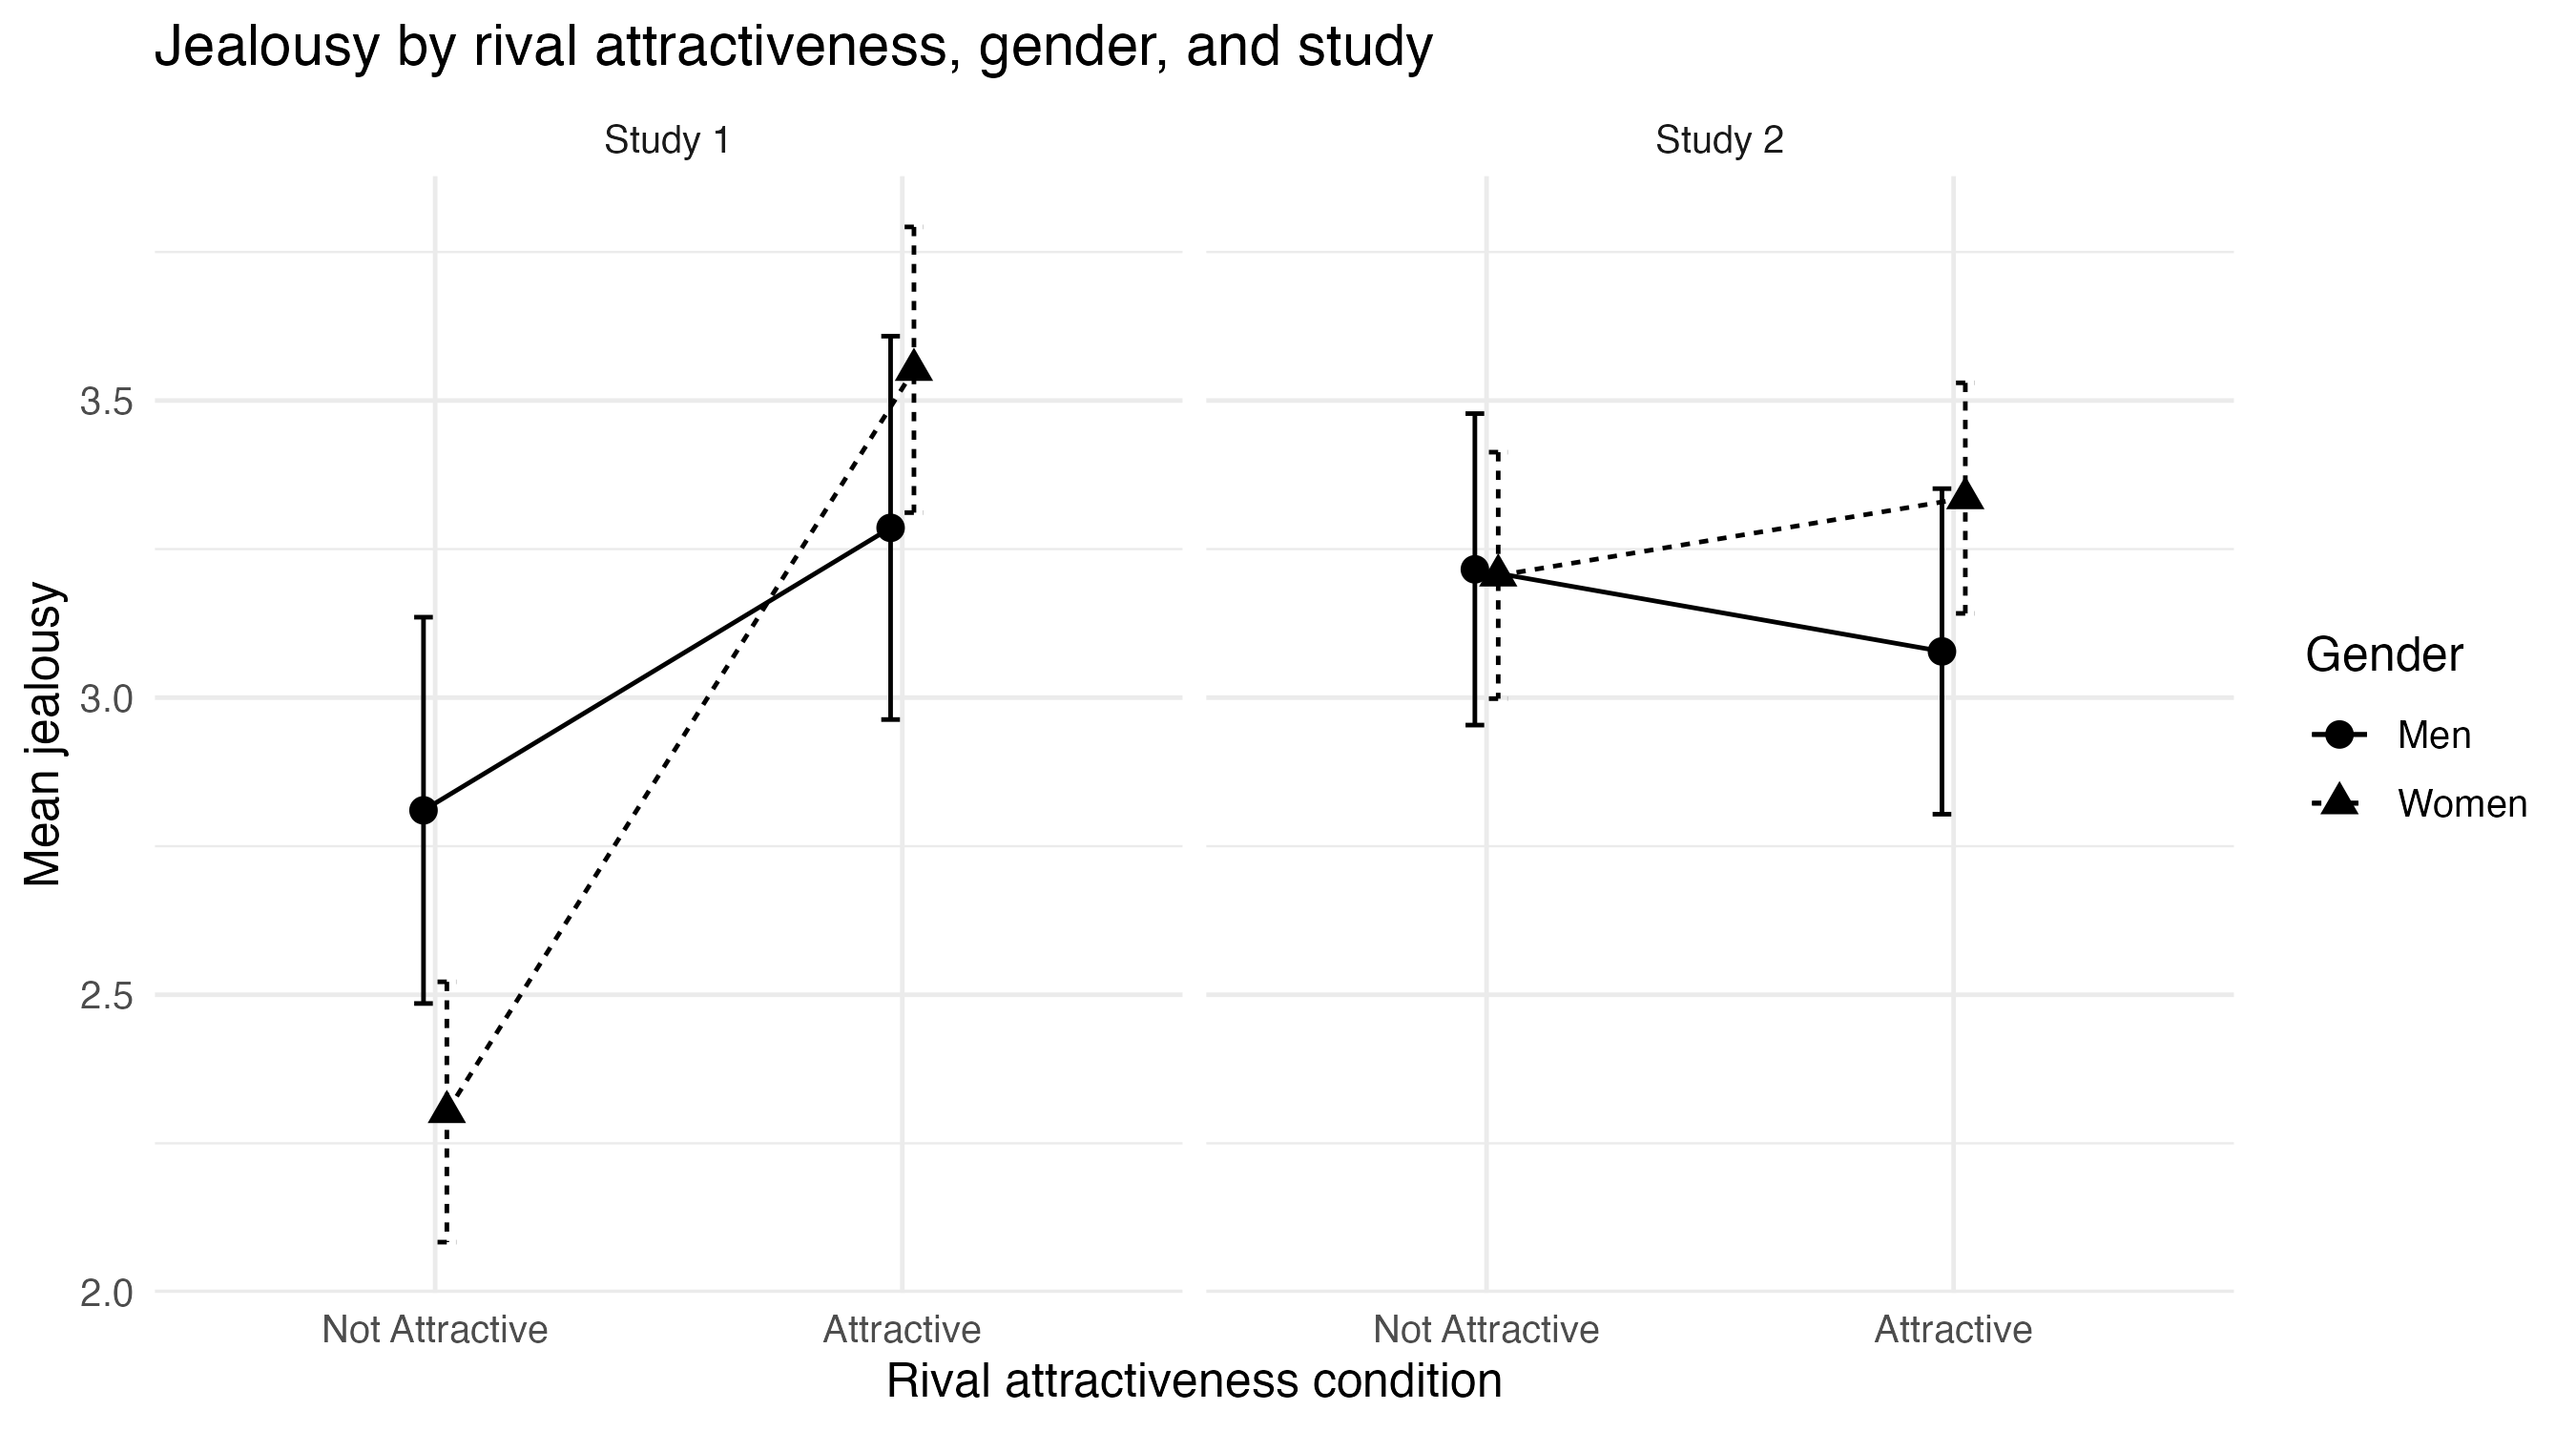
\includegraphics[width=0.8\textwidth]{extension_plot_main.png}
		\caption{Jealousy by rival attractiveness, gender, and study}
	\end{figure}
	
\begin{table}[htbp]
	\centering
	\caption{Pooled Comparison: Three-Way Interaction Effect}
	\begin{tabular}{l p{5cm} c c c c c}
		\toprule
		Study & Term & Df & Sum Sq & Mean Sq & F-value & p-value \\
		\midrule
		Pooled comparison & Study:Attractive\_condition:Gender & 1 & 2.452 & 2.452 & 1.591 & 0.208 \\
		\bottomrule
	\end{tabular}
\end{table}
	
\begin{table}[htbp]
	\centering
	\small
	\caption{Descriptive Statistics of Jealousy by Study, Gender, and Condition}
	\begin{tabular}{l l l c c c c c}
		\toprule
		Study & Gender & Attractive Condition & N & Mean & SD & SE & CI Low \\
		\midrule
		Study 1 & Men & Not Attractive & 58  & 2.81 & 1.26 & 0.166 & 2.49 \\
		Study 1 & Men & Attractive     & 56  & 3.29 & 1.23 & 0.165 & 2.96 \\
		Study 1 & Women & Not Attractive & 109 & 2.30 & 1.17 & 0.112 & 2.08 \\
		Study 1 & Women & Attractive     & 116 & 3.55 & 1.32 & 0.123 & 3.31 \\
		Study 2 & Men & Not Attractive & 88  & 3.22 & 1.25 & 0.134 & 2.95 \\
		Study 2 & Men & Attractive     & 90  & 3.08 & 1.33 & 0.140 & 2.80 \\
		Study 2 & Women & Not Attractive & 141 & 3.21 & 1.26 & 0.106 & 3.00 \\
		Study 2 & Women & Attractive     & 137 & 3.34 & 1.16 & 0.099 & 3.14 \\
		\bottomrule
	\end{tabular}
\end{table}
	
	\vspace{10cm}
	
	
	
	\subsection{Extension 2 Results}
	Figure 2 presents the predicted probability of the highest jealousy category using the ordered logit model. In Study 1, the probability increases substantially when the rival is attractive, particularly for women. In Study 2, the changes are smaller and less consistent.
	
	\begin{figure}[h]
		\centering
		
\includegraphics[width=0.8\textwidth]{ordered_logit_predicted_probability_plot.png}
		\caption{Predicted probability of the highest jealousy category}
	\end{figure}
	
	\begin{table}[htbp]
		\centering
		\caption{Comparison of OLS and Ordinal Logit Results}
		\begin{tabular}{l c c c c}
			\toprule
			Study & OLS F-value & OLS p-value & Ord. Logit Estimate & Ord. Logit p-value \\
			\midrule
			Study 1 & 7.261 & 0.0074 & 0.290 & 0.0048 \\
			Study 2 & 1.266 & 0.2612 & 0.088 & 0.3044 \\
			\bottomrule
		\end{tabular}
	\end{table}
	
	
	
	\vspace{5cm}
	
	\section{Discussion and Conclusion}
	This replication project reproduced the original study’s core jealousy models and then extended them in two methodologically relevant ways. The first extension showed that the key attractiveness-by-gender pattern is not equally strong in the two replication studies. Study 1 provides clearer support for the claim, whereas Study 2 shows a weaker pattern.
	
	The second extension showed that the same general conclusion survives re-estimation with an ordered logit model, which is more appropriate for ordinal outcome data. However, it also highlights that the effect is not uniformly large across studies.
	
	Overall, the results suggest that the original finding is not fully robust and is somewhat sample-dependent. At the same time, the consistency across modeling approaches provides some support for the underlying theoretical claim. The main contribution of this report is therefore to evaluate both robustness across samples and robustness across model specifications.
	
	
		\section{References}
		
		\textbf{Pollet TV, Saxton TK. Jealousy as a Function of Rival Characteristics: Two Large Replication Studies and Meta-Analyses Support Gender Differences in Reactions to Rival Attractiveness But Not Dominance. Pers Soc Psychol Bull. 2020 Oct;46(10):1428-1443. doi: 10.1177/0146167220904512. Epub 2020 Mar 10. PMID: 32153243; PMCID: PMC7493204.}
		
		
\end{document}
